Consider the motivating models of \cite{Spence.1973} and \cite{Ben-Porath.1967} as discussed in class.

\begin{boenumerate}
\item For both models, provide a brief description of the question they are designed to address and their key ingredients. Provide two examples of important economic features that are missing from the formal analysis?\\

\noindent{Consider the model developed in \cite{Spence.1973} in more detail. Figure \ref{Model parametrization} visualizes the information about the wage schedule and the cost of education in the parametrized model. Please assume throughout that employers belief that individuals with a level of education $y^* \geq \tfrac{5}{4}$ have a high productivity.}

\begin{figure}[h]\centering
\caption{Model parametrization}\label{Model parametrization}
\subfloat[Wage schedule]{\scalebox{0.25}{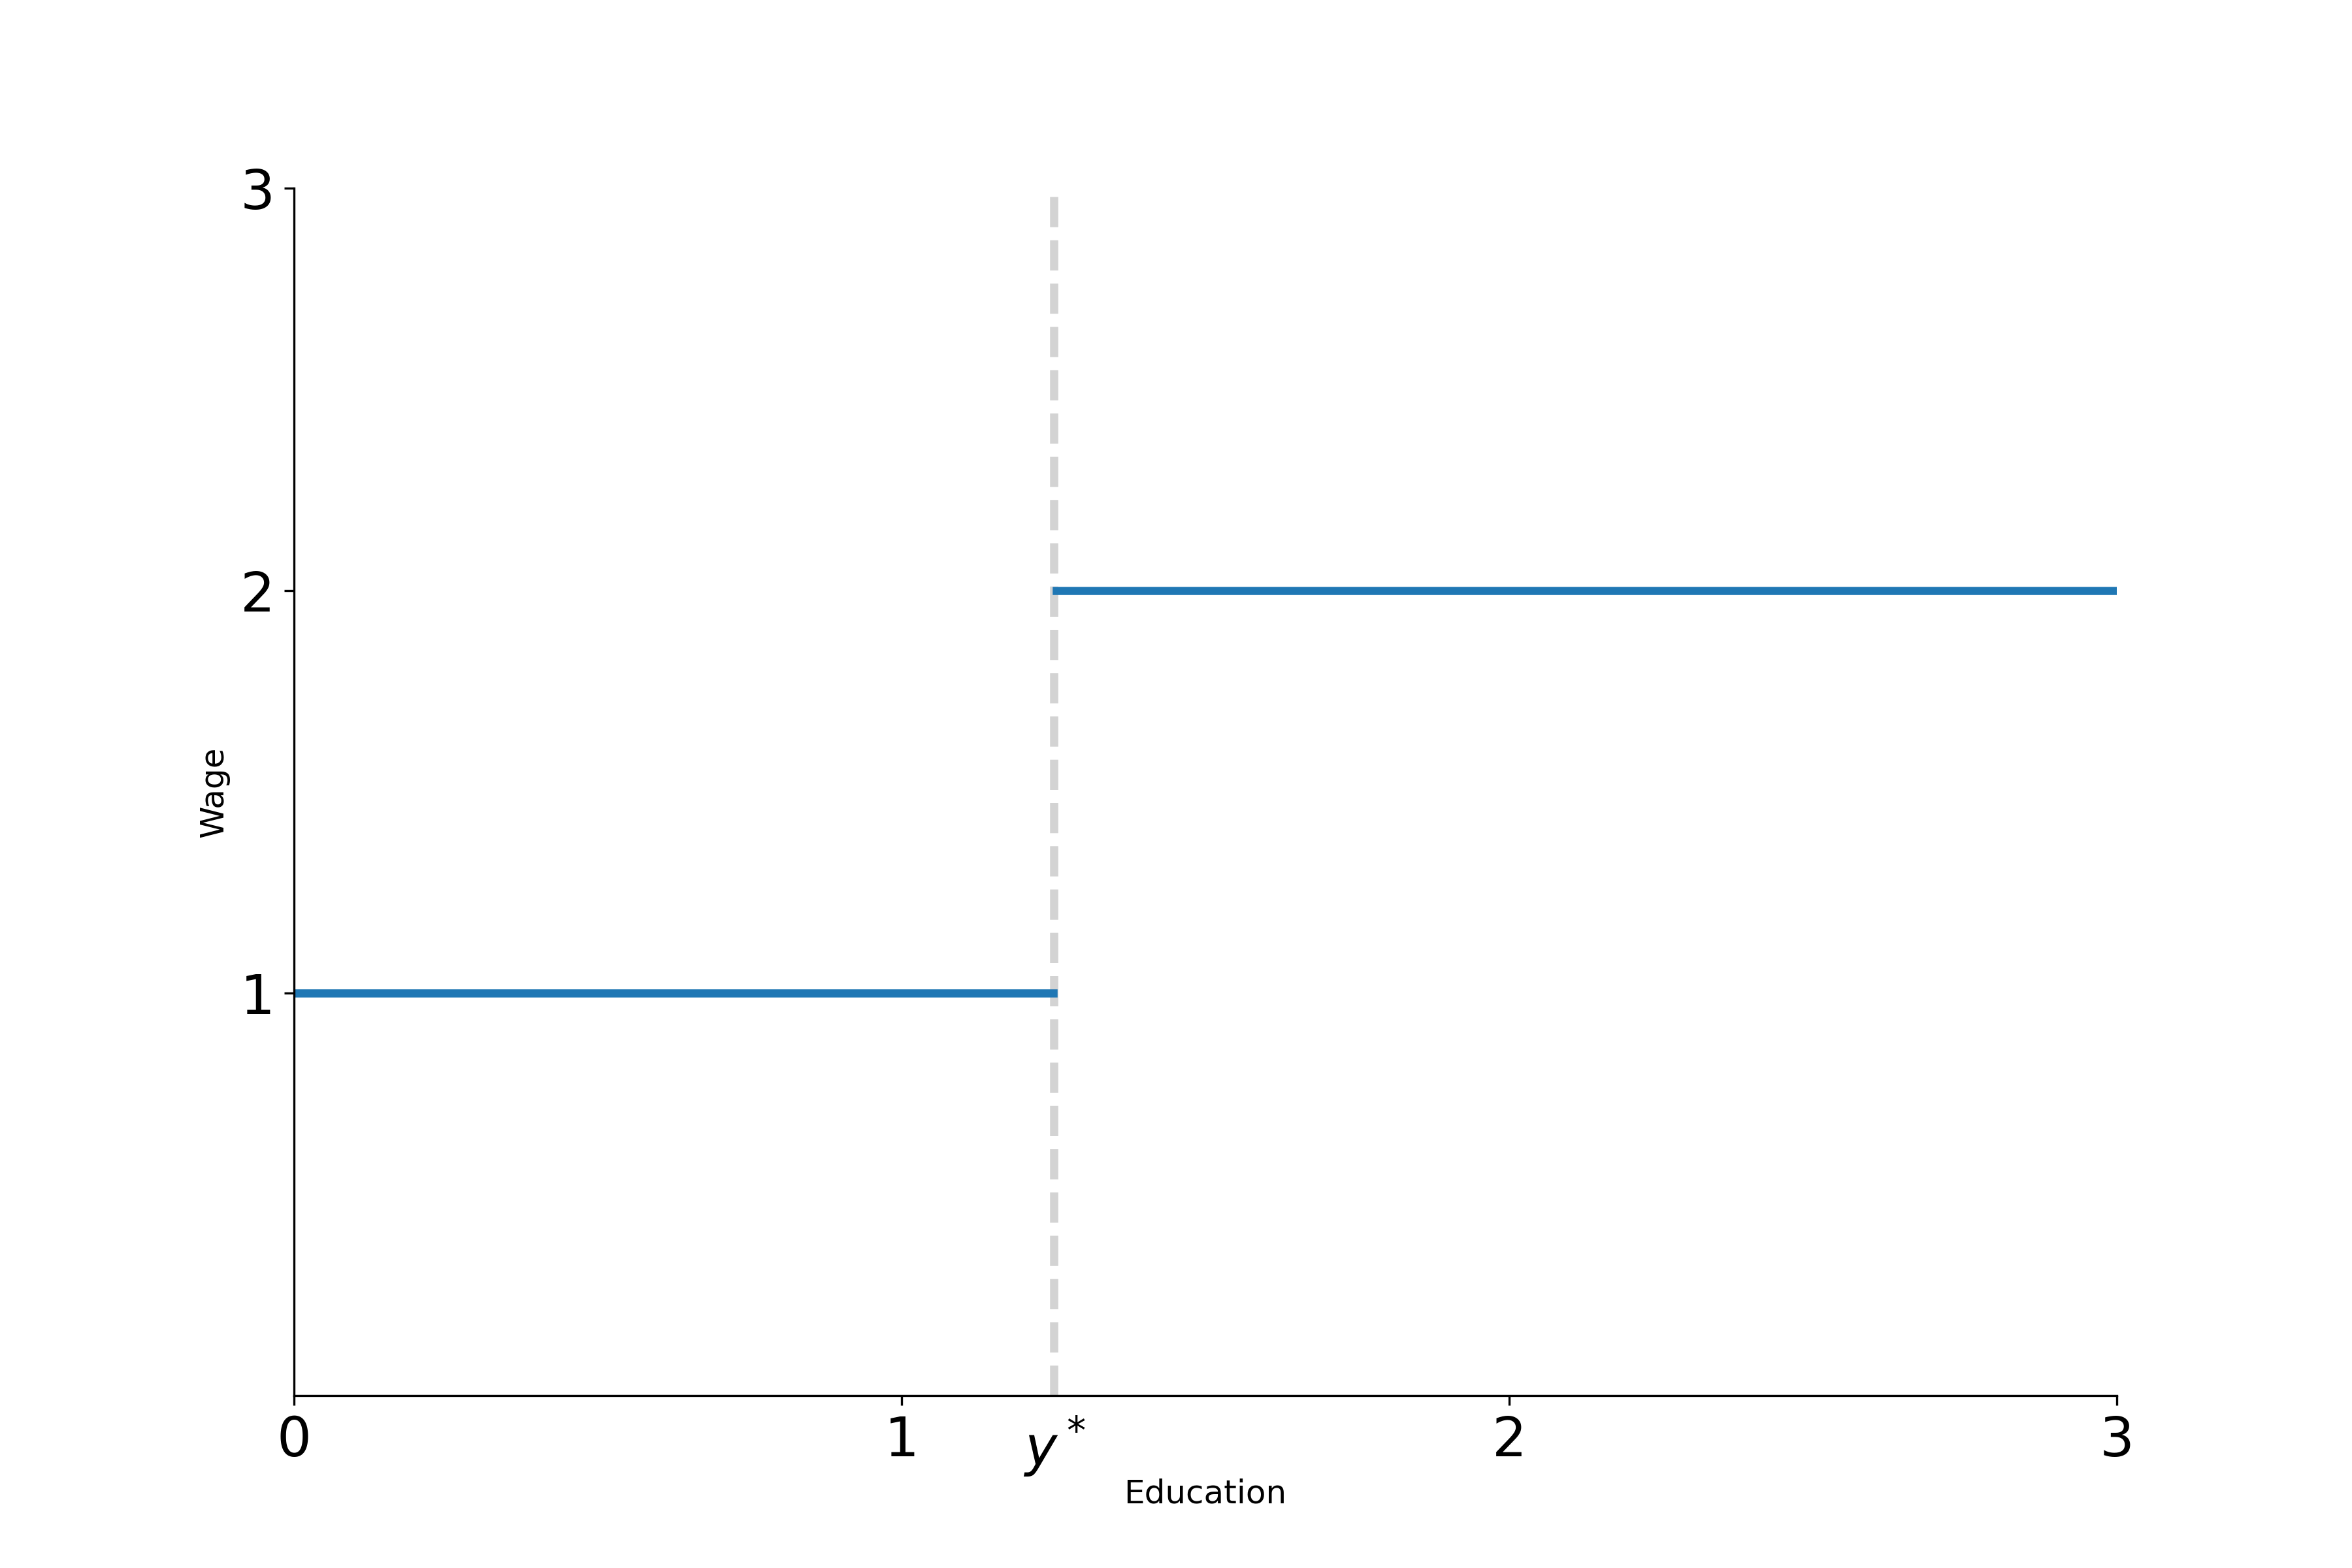
\includegraphics{fig-introduction-spence-benefit}}}
\subfloat[Cost of education]{\scalebox{0.25}{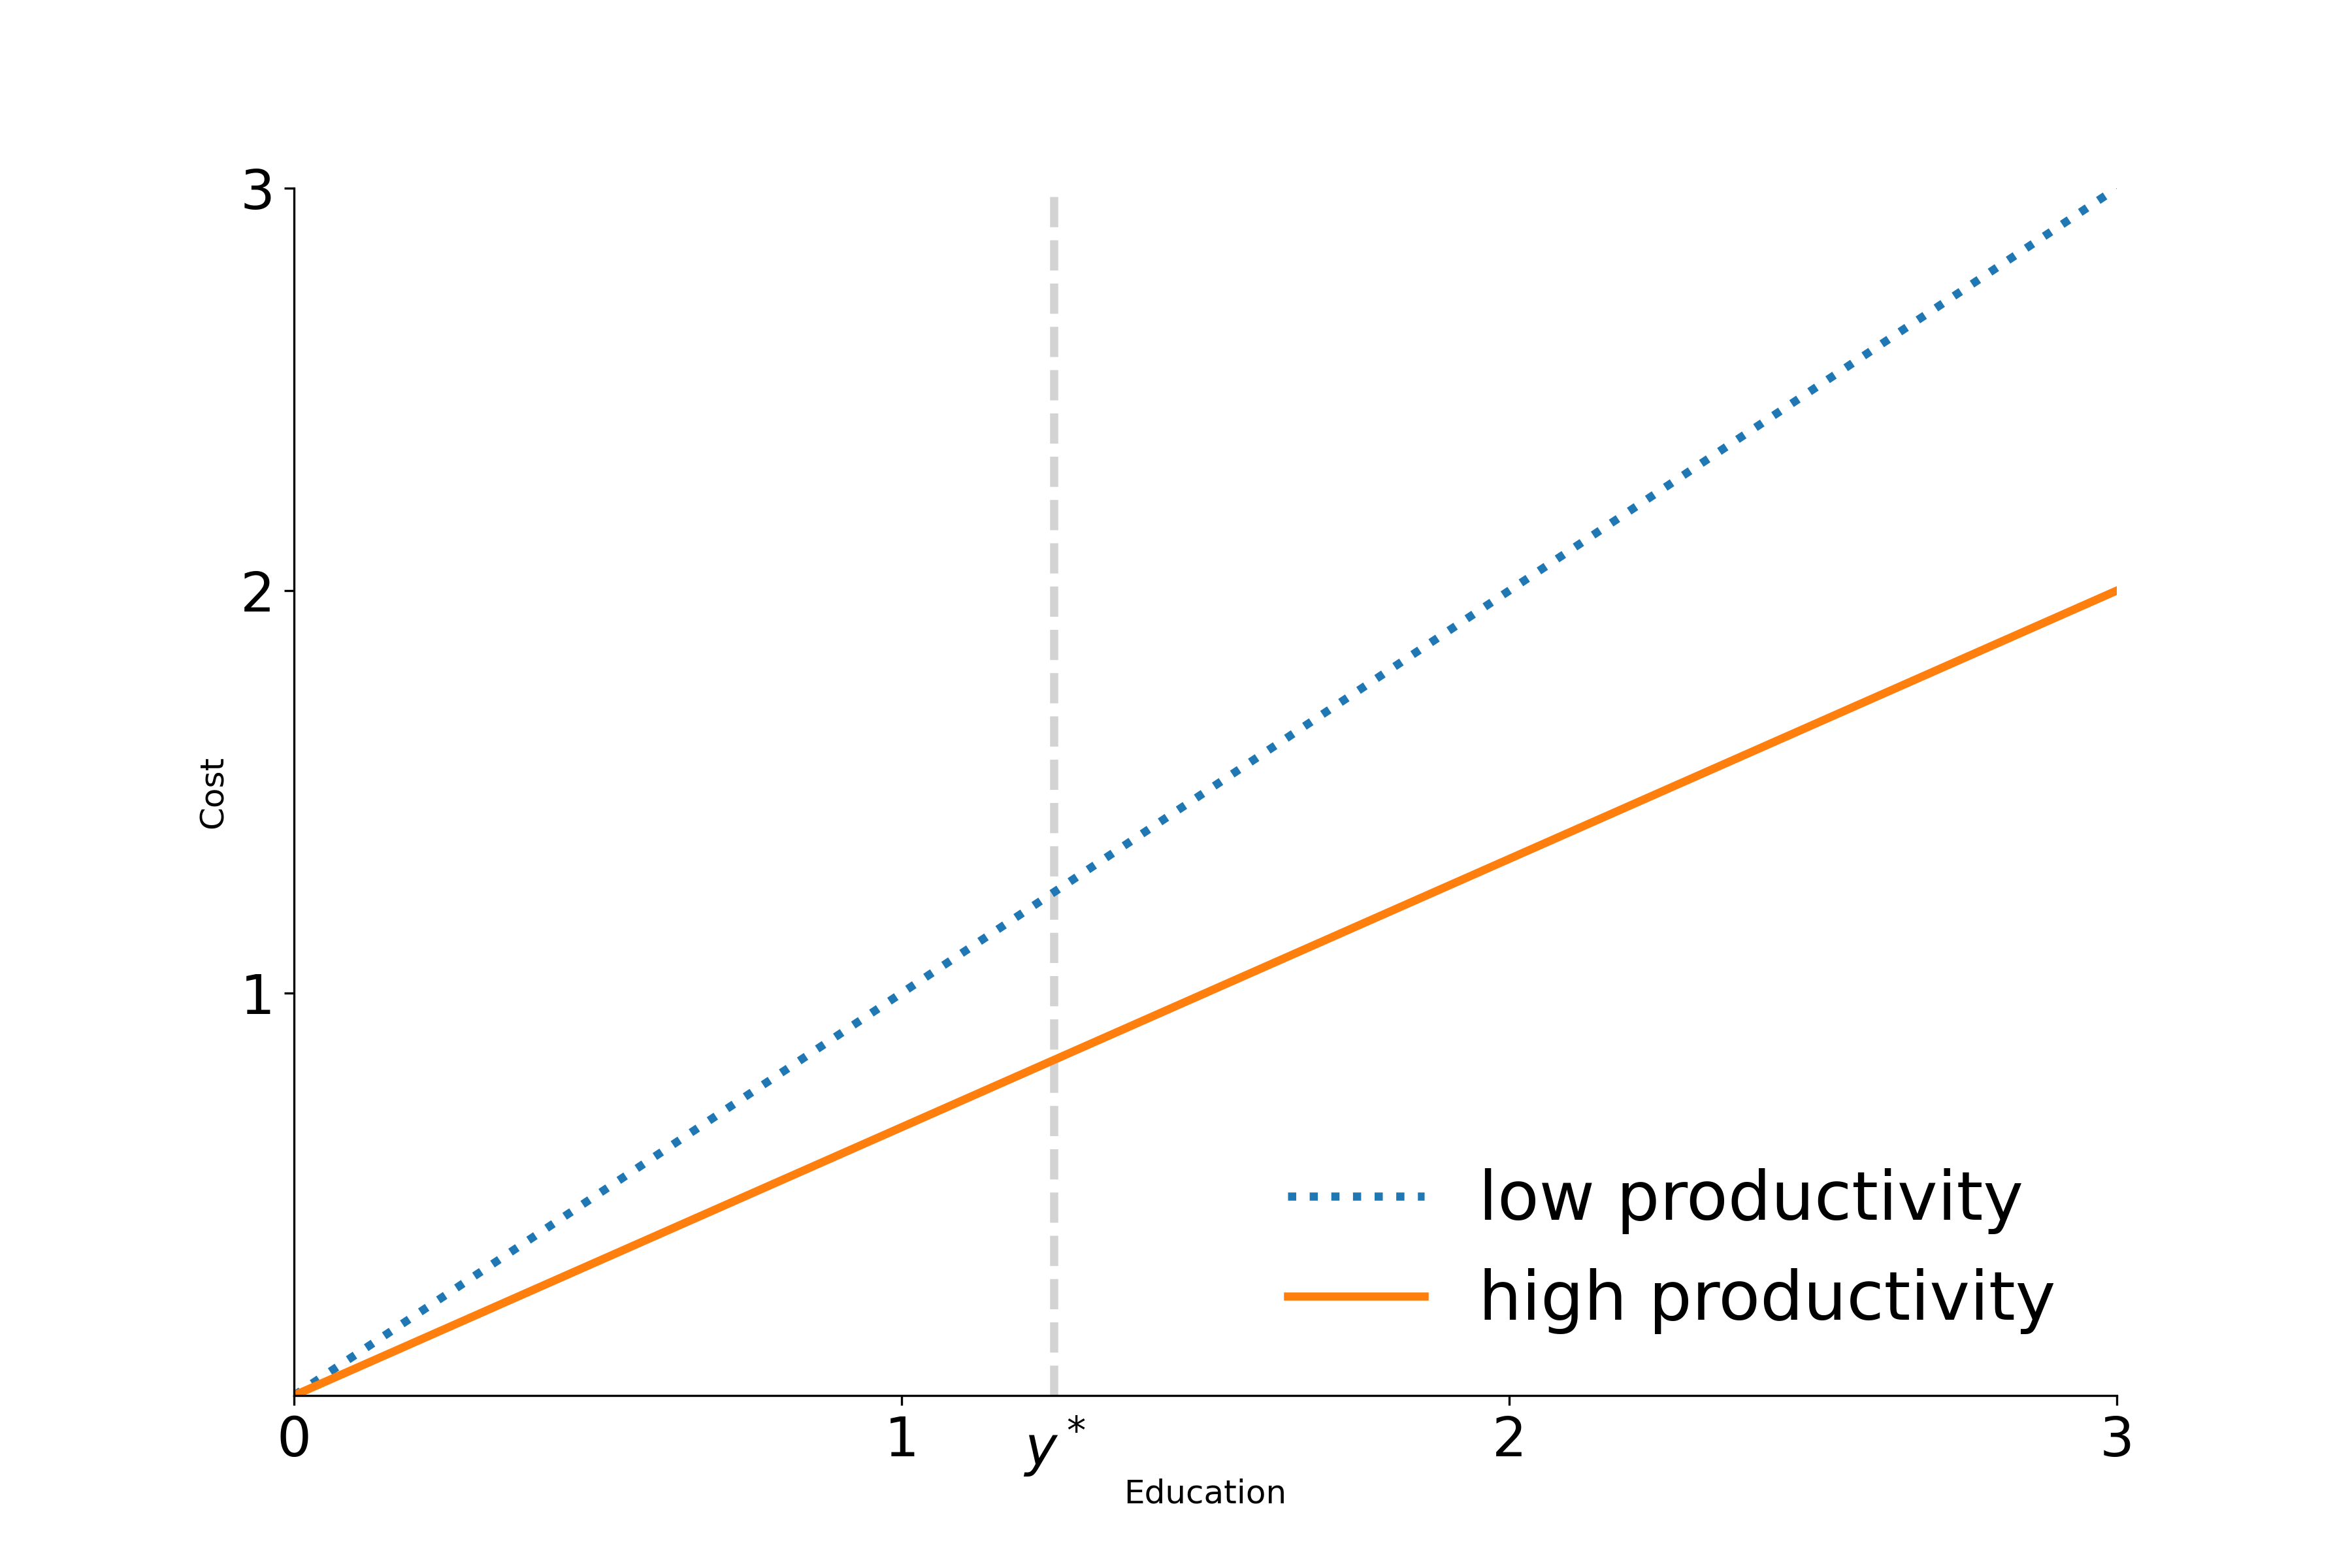
\includegraphics{fig-introduction-spence-cost}}}
\end{figure}

\item Write down the parametrization of the cost $(c_L, c_H)$ and wage $(w_L, w_H)$ functions for the high and low productivity individuals.

\item Complete Figure \ref{Canvas Surplus} by adding the surplus functions for each of the two groups over the specified range. Also, indicate the optimal level of schooling for each of the two groups.

\begin{figure}[h]\centering
\caption{Surplus of education}\label{Canvas Surplus}
\scalebox{0.35}{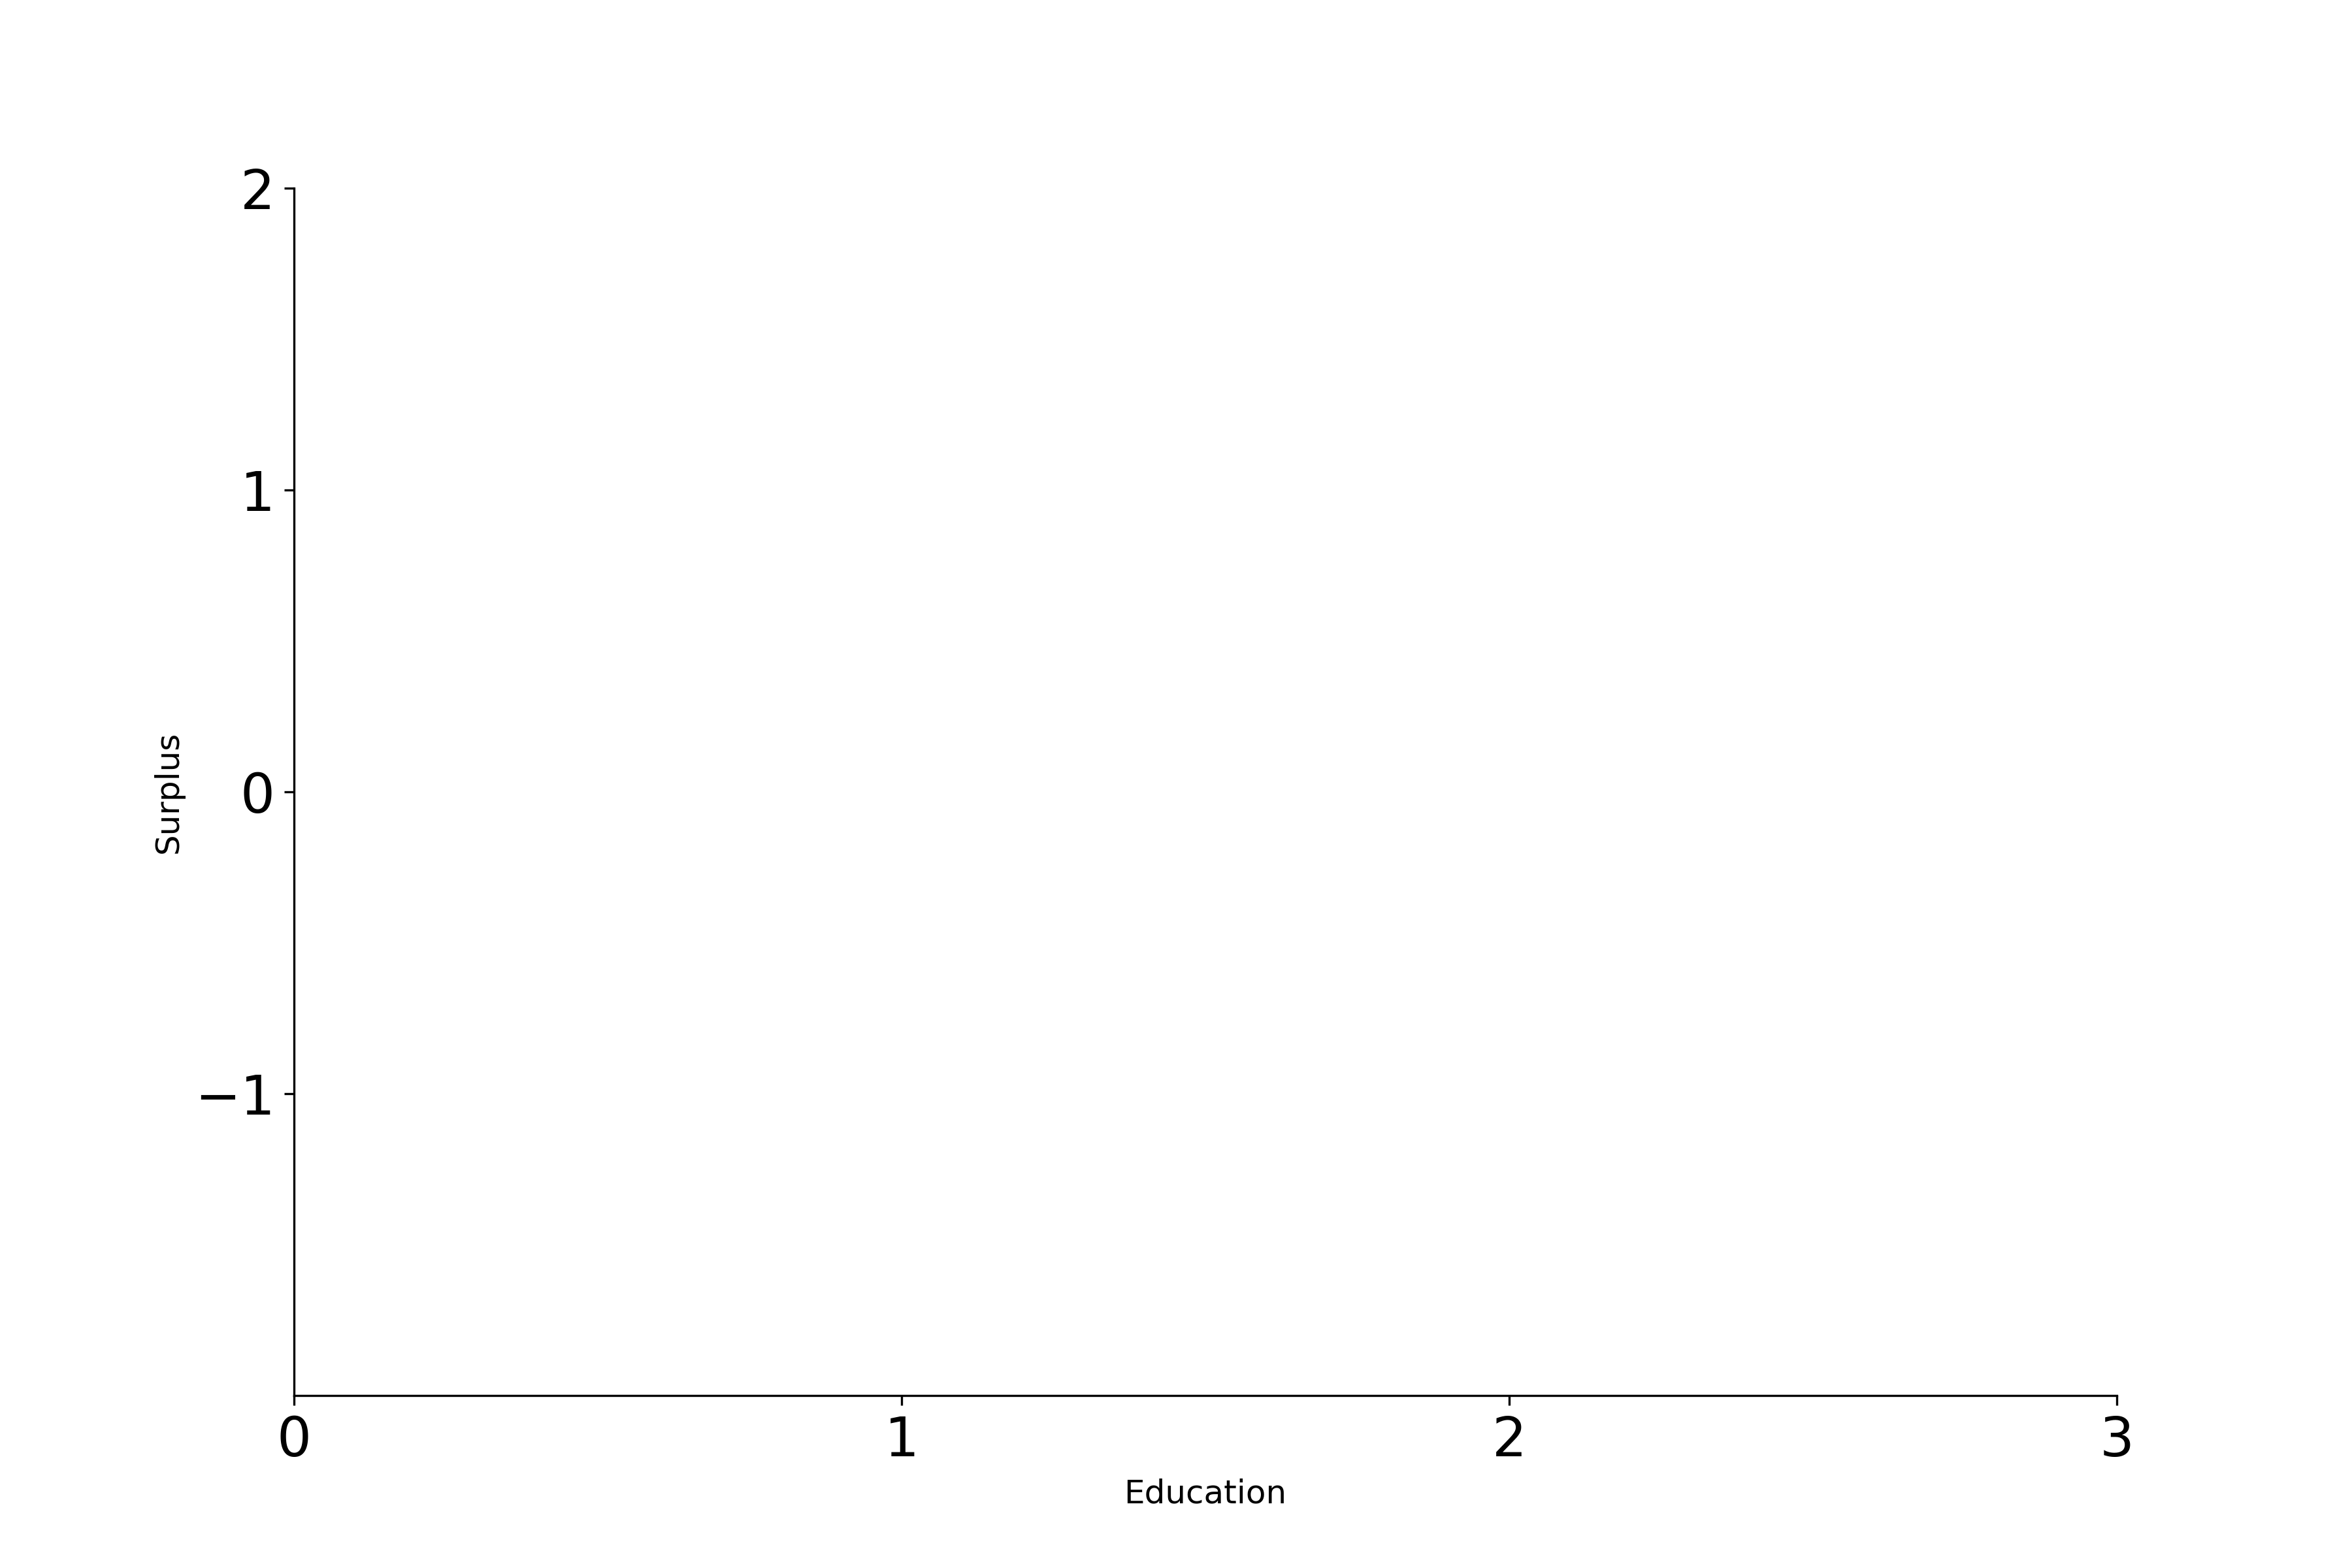
\includegraphics{fig-introduction-spence-surplus-canvas}}
\end{figure}

\item Calculate the range of the separating schooling level $y^*$ that confirms the employer's beliefs.\\

\noindent{Now consider the case where individuals do not have the ability to signal their productivity and the share of individuals with low productivity is denoted by $q_L$.\\}

\item What is the wage for each of the two groups in this scenario as a function of $q_L$?

\item  Complete Figure \ref{Canvas Market Structure} by adding the surplus and wage for the two groups under the scenario where individuals are able to signal their ability and when they are not.

\begin{figure}[h]\centering
\caption{Surplus and market structure}\label{Canvas Market Structure}
\scalebox{0.35}{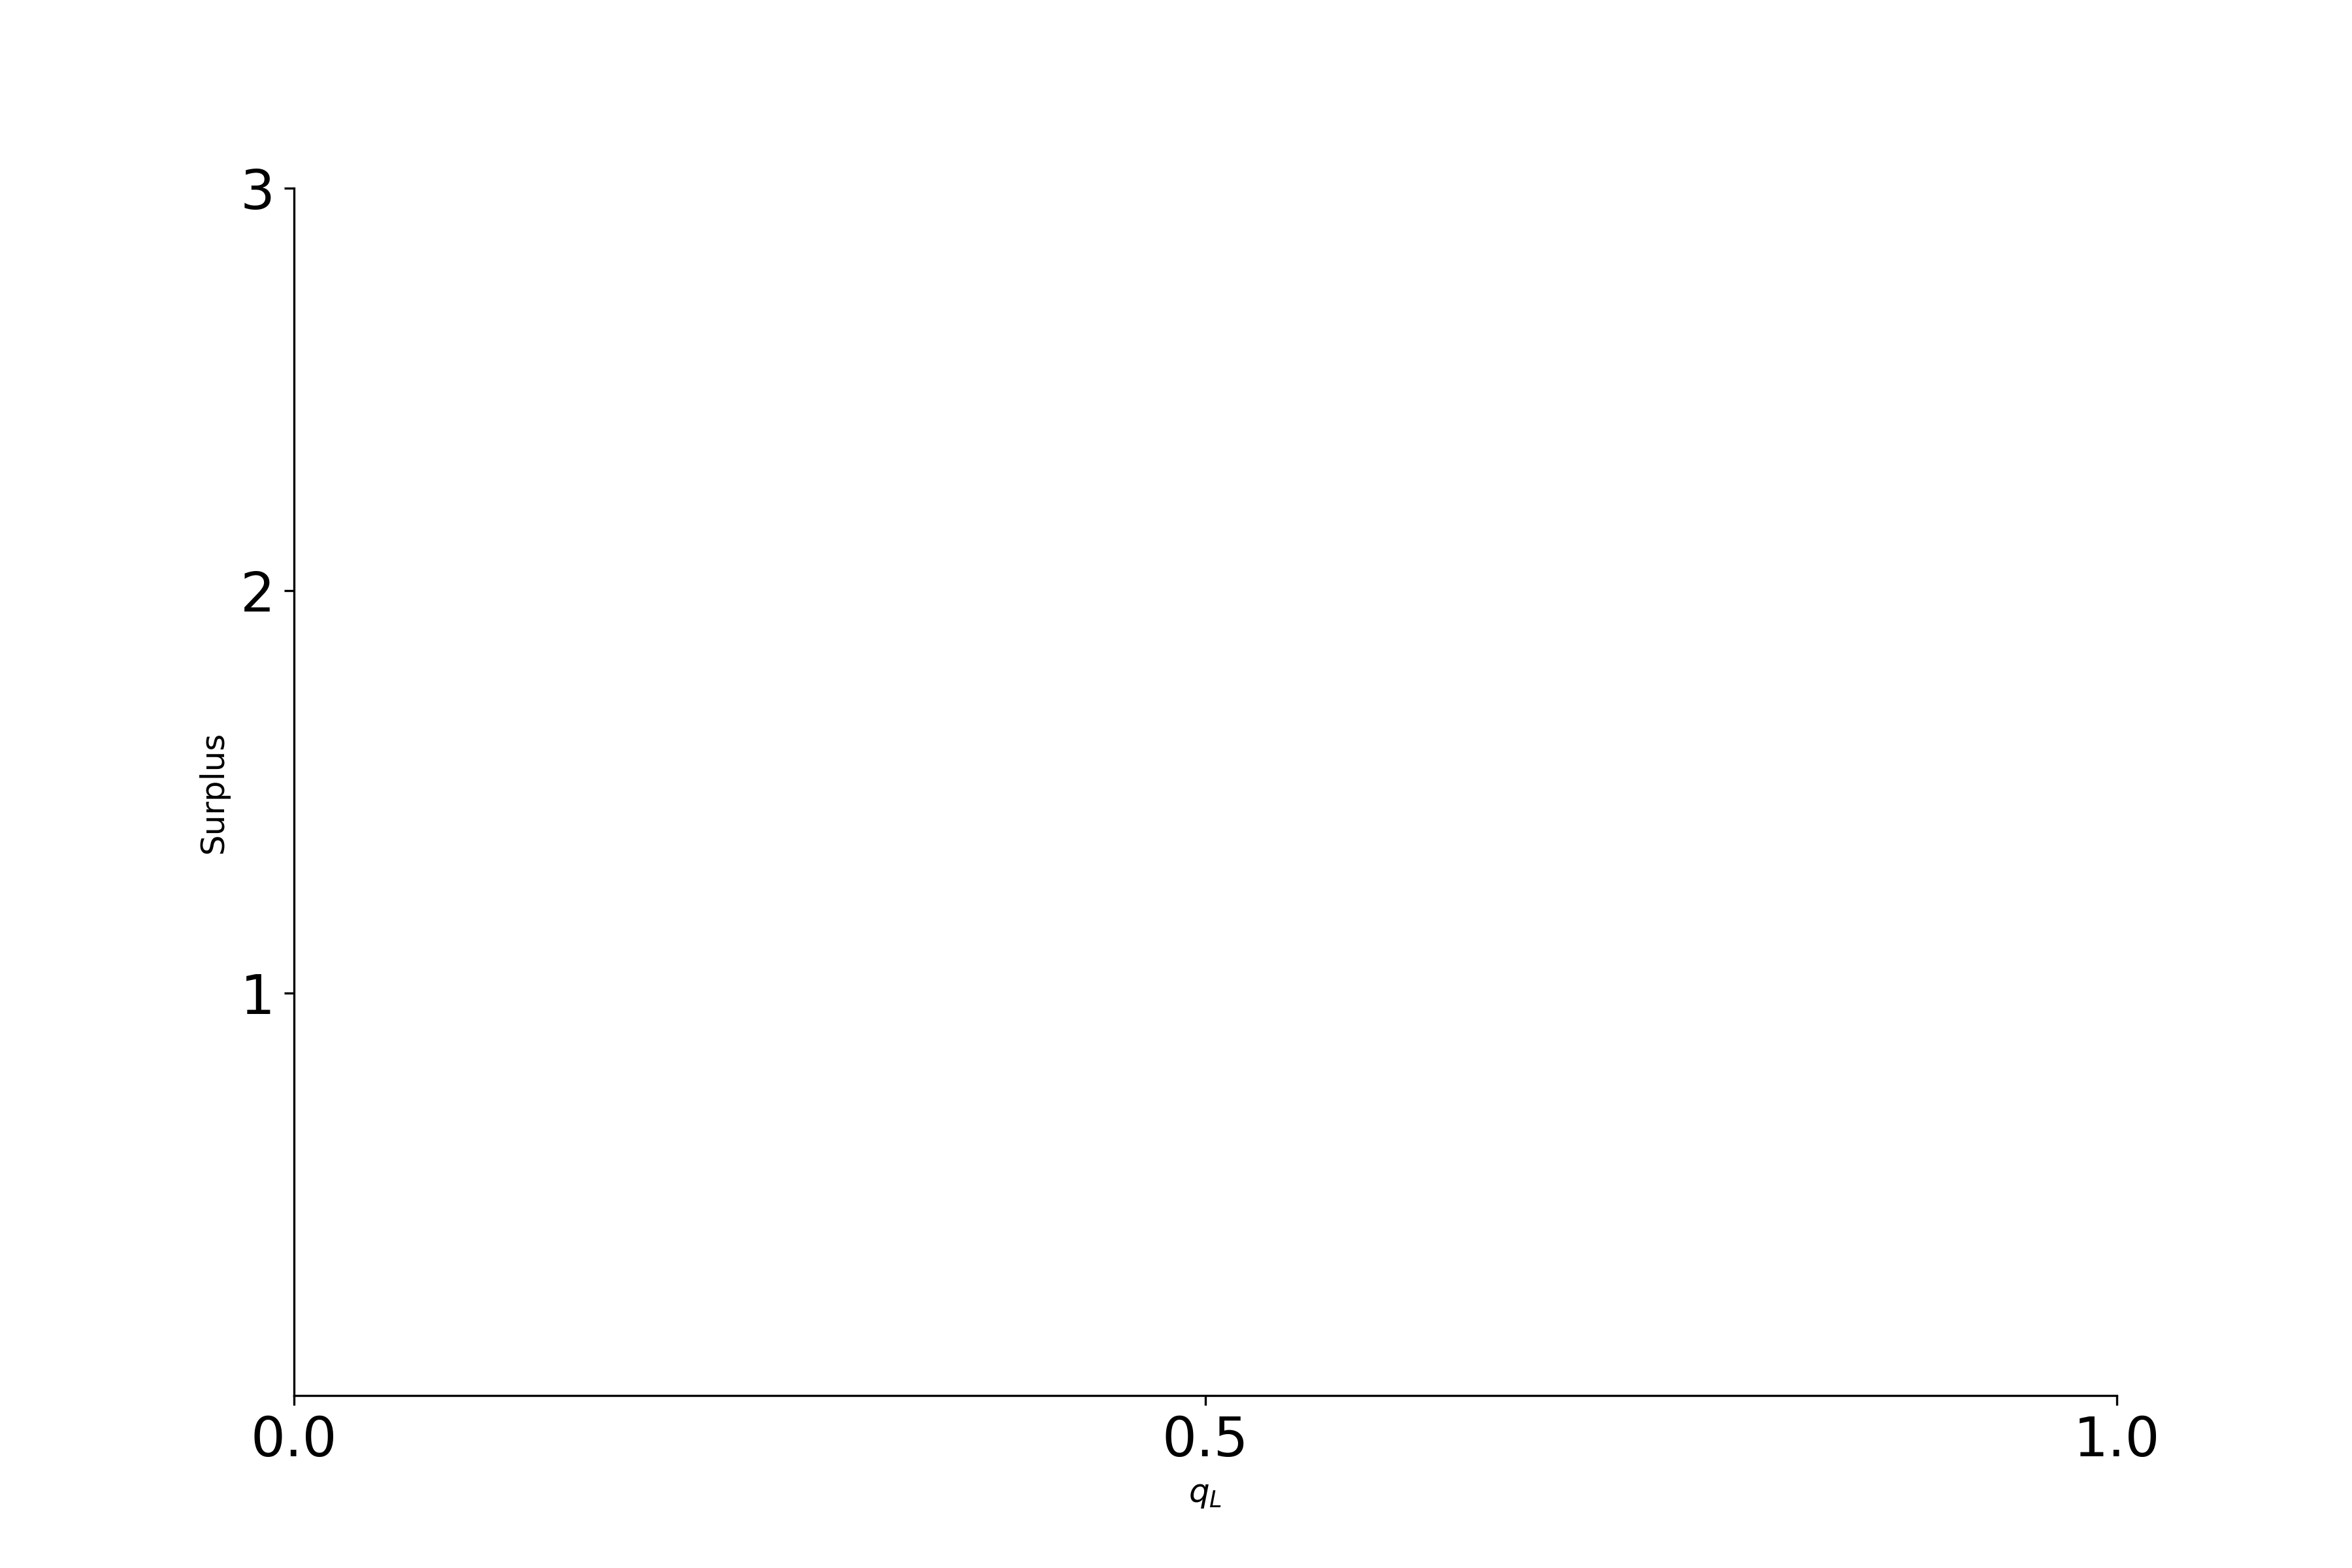
\includegraphics{fig-introduction-spence-market-structure-canvas}}
\end{figure}

\item What scenario do high productivity individuals prefer, what does their assessment depend on, when exactly do they change their mind?

\end{boenumerate}
